%-------------------------
% Resume in Latex
% Author : David
% Based on: https://github.com/jakegut/resume (which was based on https://github.com/sb2nov/resume)
% License : MIT
%------------------------

\documentclass[letterpaper,11pt]{article}

\usepackage{latexsym}
\usepackage[empty]{fullpage}
\usepackage{titlesec}
\usepackage{marvosym}
\usepackage[usenames,dvipsnames]{color}
\usepackage{verbatim}
\usepackage{enumitem}
\usepackage{fancyhdr}
\usepackage[english]{babel}
\usepackage{tabularx}
\usepackage{xcolor}
\usepackage{fontawesome5}
\usepackage{graphicx}
\usepackage{multicol}
\usepackage{enumitem}
\usepackage[margin=1in]{geometry}
\usepackage{MnSymbol,bbding,pifont}
\usepackage{ifthen}
\usepackage{calc}
\usepackage{pifont}
\usepackage{forloop}
\usepackage{eurosym}

\newcounter{starnumber}
\newcommand{\stars}[1]{
  \forloop{starnumber}{1}{\value{starnumber} < 4}{
    \ifthenelse{#1 < \value{starnumber}}{\ding{73}}{\ding{72}}%
  }
}


\input{glyphtounicode}

% -------------------- FONT --------------------
\pagestyle{fancy}
\fancyhf{} % clear all header and footer fields
\fancyfoot{}
\renewcommand{\headrulewidth}{0pt}
\renewcommand{\footrulewidth}{0pt}

% Adjust margins
\addtolength{\oddsidemargin}{-0.5in}
\addtolength{\evensidemargin}{-0.5in}
\addtolength{\textwidth}{1in}
\addtolength{\topmargin}{-1in} % Default was -.5in
\addtolength{\textheight}{1.0in}


\raggedbottom
\raggedright
\setlength{\tabcolsep}{0in}

% Section formatting
\titleformat{\section}{
  \vspace{-5pt}\scshape\raggedright\large
}{}{0em}{}[\color{black}\titlerule \vspace{-5pt}]

% Subsection formatting
\titleformat{\subsection}{
  \vspace{-4pt}\scshape\raggedright\large
}{\hspace{-.15in}}{0em}{}[\color{black}\vspace{-8pt}]

% Ensure that generate pdf is machine readable/ATS parsable
\pdfgentounicode=1

% -------------------- CUSTOM COMMANDS --------------------
\newcommand{\resumeItem}[1]{
  \item\small{
    {#1 \vspace{-2pt}}
  }
}

\newcommand{\resumeSubheading}[4]{
  \vspace{-2pt}\item
    \begin{tabular*}{0.97\textwidth}[t]{l@{\extracolsep{\fill}}r}
      \textbf{#1} & #2 \\
      \textit{\small#3} & \textit{\small #4} \\
    \end{tabular*}\vspace{-7pt}
}

\newcommand{\resumeSubSubheading}[2]{
    \item
    \begin{tabular*}{0.97\textwidth}{l@{\extracolsep{\fill}}r}
      \textit{\small#1} & \textit{\small #2} \\
    \end{tabular*}\vspace{-7pt}
}

\newcommand{\resumeProjectHeading}[2]{
    \item
    \begin{tabular*}{0.97\textwidth}{l@{\extracolsep{\fill}}r}
      \small#1 & #2 \\
    \end{tabular*}\vspace{-7pt}
}

\newcommand{\resumeSubItem}[1]{\resumeItem{#1}\vspace{-4pt}}
\newcommand{\resumeSubHeadingListStart}{\begin{itemize}[leftmargin=0.15in, label={}]}
\newcommand{\resumeSubHeadingListEnd}{\end{itemize}}
\newcommand{\resumeItemListStart}{\begin{itemize}[leftmargin=0.2in]}
\newcommand{\resumeItemListEnd}{\end{itemize}\vspace{-5pt}}

\renewcommand\labelitemii{$\vcenter{\hbox{\boldmath$\cdot$}}$}
\renewcommand\labelitemi{{\boldmath$\cdot$}}

\setlength{\footskip}{4.08003pt}

% -------------------- START OF DOCUMENT --------------------
\begin{document}

% -------------------- HEADING--------------------
% \begin{flushright}
%     \vspace{-4pt}
%     \color{gray}
%     \item
%     % Last Updated on September 9th, 2023
% \end{flushright}


\begin{minipage}{.95\linewidth}
\vspace{40pt}
\begin{center}
    \textbf{\Huge \scshape David Petri} \\ \vspace{8pt}
    \small
    % \faIcon{github}
    % \href{https://github.com/dapetri}{github.com/dapetri} $  $
    % \faIcon{code}
    % \href{https://www.dapetri.com}{dapetri.com} $  $
    % \faIcon{linkedin}
    % \href{https://linkedin.com/in/dapetri}{linkedin.com/in/dapetri} $  $
    % \faIcon{envelope}
    % \href{mailto:me@dapetri.com}{me@dapetri.com} $  $
    % \faIcon{phone}{ +49 173 7777637}
    \faIcon{envelope}
    {me@dapetri.com} $  $
    \faIcon{phone}
    {+49 173 7777637} $  $
    \faIcon{code}
    {dapetri.com} $  $
    \faIcon{linkedin}
    {linkedin.com/in/dapetri} $  $
    \faIcon{github}
    {github.com/dapetri} $  $
    % \faIcon{home}
    % {Salinenstr. 4/4, 74177 Bad Friedrichshall (DE)} $  $

\end{center}
\end{minipage}\hfill

% \begin{picture}(0,0)
    % \put(460,-9){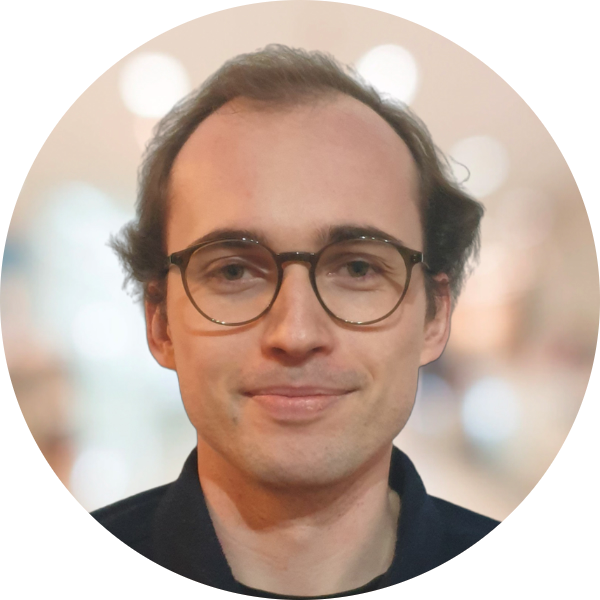
\includegraphics[width=6.5em]{img/profile-pic-2.png}}
% \end{picture}


%
% -------------------- EXPERIENCE --------------------
\section{Experience}
\resumeSubHeadingListStart
\vspace{5pt}
\resumeProjectHeading
{\textbf{ML Engineer (Computer Vision \& IoT)} \space $|$ \space Schwarz IT -- Heilbronn, Germany\vspace{8pt}}{Mar. 2024 -- \textit{present}}
\textit{\small{Python, C/C++, Docker, Kubernetes, CI/CD, Azure, Git}}
\vspace*{-5pt}
\resumeItemListStart
\resumeItem{\textbf{Led} a junior development team of three machine learning and software engineers}
\vspace{7pt}
\resumeItem{Industrialized \textbf{large-scale anomaly detection microservices (+300)} for material jams on conveyorbelts in PreZero waste sorting plants}
\resumeItem{\textbf{Prevented a \EUR{74k} loss} in production downtime within the first two months of deployment}
\vspace{7pt}
\resumeItem{Industrializing a \textbf{ResNet-8}-based meat classificator for a Kaufland meat factory}
\resumeItem{Substituting two workers per shift -- \textbf{cutting production costs} by \textbf{\EUR{1200}/day}}
\resumeItemListEnd

\vspace{12pt}

\resumeProjectHeading
{\textbf{SDE \& Co-Founder} \space $|$ \space Haimdall \space  [haimdall.org] \space \vspace{8pt}}{May 2024 -- \textit{present}}
\textit{\small{Python, Flask, Flutter, Dart, RestAPI, Docker, Git}}
\vspace*{-5pt}
\resumeItemListStart
\resumeItem{Full-stack development of a \textbf{mobile alerting app} for first aiders on larg-scale events}
\resumeItemListEnd

\vspace{12pt}
\resumeProjectHeading
{\textbf{ML Engineer (Computer Vision)} \space $|$ \space BMW Group -- Munich, Germany\vspace{8pt}}{Nov. 2023 -- Mar. 2024}
\textit{\small{Python, PyTorch, OpenCV, Anomalib, Git}}
\vspace*{-5pt}
\resumeItemListStart
% \resumeItem{Development and implementation of a \textbf{data preprocessing pipeline} for a \textbf{first-of-a-kind industrial labeled dataset}.}
\resumeItem{Piloted a \textbf{ResNet} embedding-based \textbf{anomaly detection} algorithm for production errors on V8 engine blocks}
\resumeItem{Initialized the \textbf{process integration} of \textbf{AI-supported error detection} for the quality inspectors}
\resumeItemListEnd

\vspace{12pt}
\resumeProjectHeading
{\textbf{ML Researcher \& SDE (Work Study)} \space $|$ \space Karlsruhe Institute of Technology, Germany\vspace{8pt}}{Apr. 2023 -- Nov. 2023}
\textit{\small{Python, PyTorch, WandB, Git}}
\vspace*{-5pt}
\resumeItemListStart
\resumeItem{Developed a \textbf{GNN}-based \textbf{generative adversarial imitation/reinforcement learning} algorithm to learn adaptive mesh refinement strategies for the finite element method to approximate partial differential equations}
\resumeItem{Laid a foundation for the follow-up paper arXiv:2406.14161}
% \resumeItem{Developed a \textbf{GNN} based \textbf{imitation/reinforcement learning} algorithm to learn \textbf{Adaptive Mesh Refinement} strategy for the \textbf{Finite Element Method} through expert demonstrations and preferences by using \textbf{Generative Adversarial Imitation Learning} to train the \textbf{Proximal Policy Optimization} \textbf{Reinforcement Learning} algorithm.}
% \resumeItem{Achieved a \textbf{91\% coverage} with the expert strategy distribution.}
\resumeItemListEnd

% \vspace{5pt}
% \resumeProjectHeading
% % {\textbf{Machine Learning Researcher Intern} $|$ \footnotesize\emph{Karlsruhe Institute of Technology}\space [\href{https://github.com/alr-internship/self-supervised-depth-denoising}{\color{blue}{GitHub}}, \href{https://arxiv.org/abs/2305.05778}{\color{blue}{arXiv}}]\vspace{8pt}}{Oct. 2021 -- Apr. 2022}
% {\textbf{Machine Learning Researcher Intern} $|$ \footnotesize\emph{Karlsruhe Institute of Technology}\vspace{8pt}}{Oct. 2021 -- Apr. 2022}
% {\small Python, PyTorch (Vision), OpenCV, Open3D, NumPy, Git}
% \vspace*{-5pt}
% \resumeItemListStart
% \resumeItem{Developed and implemented a \textbf{data preprocessing pipeline} to \textbf{record, transform} and \textbf{mask 3D images}.}
% \resumeItem{Trained a \textbf{Deep Convolutional Neural Network} for \textbf{denoising depth-maps of 3D images}.}
% \resumeItem{Achieved a \textbf{60\% reduction of noise} in the depth images.}
% \resumeItemListEnd

\vspace{12pt}
\resumeProjectHeading
% {\textbf{Software Developer Freelance} $|$ \footnotesize\emph{Kuori Materials, Basel (CH)}\space [\href{https://www.kuori-materials.com/}{\color{blue}{kuori.ch}}]\vspace{8pt}}{May 2021 -- Aug. 2021}
{\textbf{SDE} \space $|$ \space Kuori Materials -- Basel, Switzerland \space  [kuori.ch] \vspace{8pt}}{May 2021 -- Aug. 2021}
\textit{\small React, TypeScript, Git}
\resumeItemListStart
\resumeItem{Developed the frontend for the company's homepage}
\resumeItemListEnd
\vspace*{-5pt}
% \resumeItemListStart
% \resumeItem{Developed the company's ebsite according to specifications of the design department.}
% % \resumeItem{Successfully \textbf{deployed} and \textbf{maintained} the \textbf{first internet presence} of the company.}
% \resumeItemListEnd

\resumeSubHeadingListEnd
\vspace{5pt}

% -------------------- publications --------------------
\section{Publications}

% \resumeItem{\textbf{Multi-Object Self-Supervised Depth Denoising} [Kienle \& Petri, 2023, \href{https://arxiv.org/abs/2305.05778}{\color{blue}{arXiv: 2305.05778}}]}

\resumeSubHeadingListStart
\vspace{5pt}
\resumeProjectHeading
{\textbf{Multi-Object Self-Supervised Depth Denoising} \space {[Kienle \& Petri, 2022, arXiv:2305.05778]}\vspace{8pt}}{}
{\small{Python, PyTorch, OpenCV, Open3D, Git}}
\vspace*{-5pt}
\resumeItemListStart
\resumeItem{Developed a \textbf{data preprocessing pipeline} to record, transform and mask \textbf{3D images}}
\resumeItem{Trained a \textbf{U-Net} for \textbf{denoising 3D images} achieving a \textbf{60\% reduction in depth-noise}}
\resumeItemListEnd

\resumeSubHeadingListEnd

\vspace*{-5pt}

% -------------------- skills --------------------
% \section{Skills}
% \vspace*{-13pt}
% \begin{itemize}[leftmargin=0.15in, label={}]
%     \small{\item{
%         \begin{multicols}{4}
%             \begin{itemize}[leftmargin=0in, label={}]
%                 \item \textbf{Prog. Languages}
%                 \begin{itemize}[leftmargin=0.15in, label={\textbf{·}}]
%                     \item Python \stars{3}
%                     \item SQL \stars{3}
%                     \item Java \stars{2}
%                     \item Dart \stars{1}
%                     \vfill\null
%                     \columnbreak
%                 \end{itemize}

%                 \item \textbf{Libraries}
%                 \begin{itemize}[leftmargin=0.15in, label={\textbf{·}}]
%                     \item PyTorch \stars{2}
%                     \item OpenCV \stars{2}
%                     \item Open3D \stars{1}
%                     \vfill\null
%                     \columnbreak
%                 \end{itemize}

%                 \item \textbf{Tools/Frameworks}
%                 \begin{itemize}[leftmargin=0.15in, label={\textbf{·}}]
%                     \item Git \stars{3}
%                     \item Docker \stars{2}
%                     \item Flask \stars{1}
%                     \item Flutter \stars{1}
%                     \vfill\null
%                      \columnbreak
%                 \end{itemize}

%                 \item \textbf{Spoken Languages}
%                 \begin{itemize}[leftmargin=0.15in, label={\textbf{·}}]
%                     \item German: \textit{native}
%                     % \item English: \textit{C2} - TOEFL 114/120
%                     \item English: \textit{C2}
%                     \item Italian: \textit{B2}
%                     % \item Spanish: \textit{B1}
%                     % \item French: \textit{B1} - DELF
%                     % \item Hungarian: \textit{A2}
%                      \vfill\null
%                      \columnbreak
%                 \end{itemize}
%             \end{itemize}
%         \end{multicols}
%     }}
% \end{itemize}
% \vspace*{-30pt}


% \begin{itemize}[leftmargin=0.15in, label={}]
%     \small{\item{
%                     \begin{tabbing}
%                         \textbf{Pragramming Languages} ~~~ \={Python (\textit{Proficient}), Java (\textit{Intermediate}), SQL (\textit{Proficient}), TypeScript (Beginner)} \\
%                         \textbf{Libraries} \> {PyTorch (3 Y.), OpenCV, Open3D, NumPy, SciPy, Pandas, Matplotlib} \\
%                         \textbf{Tools/Frameworks} \> {Git (4 Y.), Docker (2 Y.), React (2 Y.)} \\
%                         \textbf{Spoken Languages} \> {German: \textit{native},\quad English: \textit{C2} - TOEFL 114/120},\ \\ \> Italian: \textit{B2},\quad \quad \quad  Spanish: \textit{B1},\quad French: \textit{DELF B1},\quad Hungarian: \textit{A2}

%                         % \textbf{Certificates} \> {AWS Certified Cloud Practitioner}


%                     \end{tabbing}
%                 }}
% \end{itemize}
% -------------------- EDUCATION --------------------
% \vspace*{-30pt}
% \section{Education}
% \resumeSubHeadingListStart

% \resumeProjectHeading
% {\textbf{M.Sc. Computer Science} \space $|$ \space KIT* -- Germany\hspace{81.5pt}DE 1.4, US 3.8, CH 5.6 \hspace{5pt} \textbf{top 10\%}}{2021--2023}

% \resumeProjectHeading
% {\textbf{B.Sc. Computer Science} \space $|$ \space KIT* -- Germany\hspace{84pt}DE 2.0, US 3.5, CH 5.0 \hspace{5pt}}{2018--2021}

% \resumeProjectHeading
% {\textbf{B.Sc. Business and Economics} \space $|$ \space JGU** -- Germany\hspace{43.5pt} DE 1.9, US 3.5, CH 5.1 \space}{2015--2018}

% \vspace*{5pt}
% \resumeSubHeadingListEnd

\section{Education}
\vspace{5pt}
\resumeSubHeadingListStart

\resumeProjectHeading
{\textbf{M.Sc. Computer Science} \space $|$ \space Karlsruhe Institute of Technology, Germany --  \textbf{top 10\%}}{2021--2023}

\resumeProjectHeading
{\textbf{B.Sc. Computer Science} \space $|$ \space Karlsruhe Institute of Technology, Germany \hspace{5pt}}{2018--2021}

\resumeProjectHeading
{\textbf{B.Sc. Business and Economics} \space $|$ \space Johannes Gutenberg University of Mainz, Germany\hspace{43.5pt} \space}{2015--2018}

\vspace*{5pt}
\resumeSubHeadingListEnd

% \resumeSubHeadingListStart

% \resumeSubheading
% {\small B.Sc. + M.Sc. Computer Science}{2021 - 2023}
% {Karlsruhe Institute of Technology (DE)}{GPA: \textbf{top 10\%} - DE \textbf{1.4}, US 3.8, CH 5.6}

% \vspace{3pt}

% \resumeSubheading
% {B.Sc. Computer Science}{2018 - 2021}
% {Karlsruhe Institute of Technology (DE)}{GPA: DE 2.0, US 3.5, CH 5.0}

% \vspace{3pt}

% \resumeSubheading
% {B.Sc. Business \& Economics}{2015 - 2018}
% {Johannes Gutenberg University Mainz (DE) /}{GPA: DE 1.9, US 3.5, CH 5.1}

% \vspace{2pt}
% \textit{\small Ca'Foscari University of Venice (IT)}

% \vspace{2pt}
% \begin{tabular*}{0.7\textwidth}{@{\hskip 0.1in}l@{\hskip 0.1in}l}
%     {\small \textbf{\textit{Coursework:}}} & {\small Machine Learning, Deep Learning, Neural Networks, Computer Vision, Distributed \& Scalable AI,} \\
%     {\space} & {\small Statistics, Optimization Methods, Reinforcement Learning, Robotics, Telematics}
% \end{tabular*}\vspace{-7pt}



% \resumeSubHeadingListEnd


% % -------------------- PROJECTS --------------------
% \vspace{-10pt}
% \section{Hobbies}
% \begin{tabular}{ l l l}

%     % \quad \small · Chess:  Elo $\sim$ 1550 [\href{https://lichess.org/@/DaPetri}{lichess}] &\small \quad · Learning new languages \\
%     \quad \small · Chess:  Elo $\sim$ 1550 \quad \quad \quad &\small \quad · Learning new languages \quad \quad · \small Play Basketball \quad \quad · Refurbishing Old-Timer Motorbikes
%     % \quad · \small Basketball &\small \quad · Refurbishing Old-Timer Motorbikes \\
% \end{tabular}

% \lfoot{
% \footnotesize\emph{* KIT = Karlsruhe Institute of Technology }\\
% \footnotesize\emph{** JGU = Johannes Gutenberg University Mainz}
% }




\end{document}
